\subsubsection{Динамическая подсветка}
Современные IDE однако могут осуществлять статическим образом, но и на основе некоторой контекстной информации. Например, если каретка курсора располагается непосредственно перед открывающей скобкой, то эта скобка и парная ей закрывающая скобка могут быть особо выделены цветом. В данной работе такая возможность также реализована. 

В такой задаче уже не все предположение, сделанные в случае статической подсветки, применимы. Добавим в грамматику арифметических выражений правило 

expr : LBRACE expr RBRACE

и рассмотрим вход, изображённый на рисунке ~\ref{dynamic_idea}. 

\begin{figure}[h]
\centering
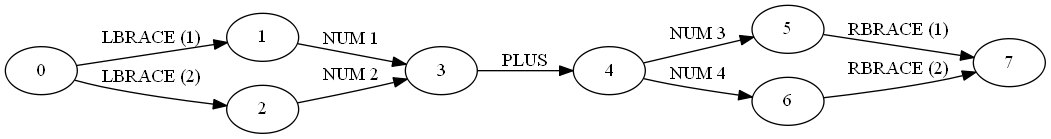
\includegraphics[width=150mm]{Pictures/Dynamic_Idea.png}
\caption{Пример получения SPPF из нескольких деревьев.}
\label{dynamic_idea}
\end{figure}

Алгоритм, предложенный в предыдущем разделе, вернёт деревья, изображённые на рисунке ~\ref{staticRes}.

\begin{figure}[h]
    \centering
    \begin{subfigure}[h]{0.25\textwidth}
         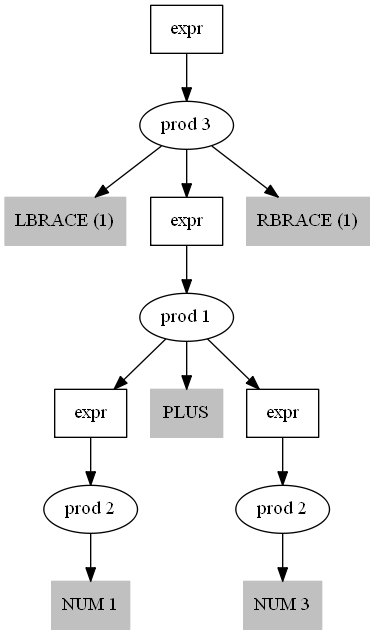
\includegraphics[height=100mm]{Pictures/Dynamic_StaticRes1.png}
    \end{subfigure}
    \qquad \qquad
    \begin{subfigure}[h]{0.25\textwidth}
         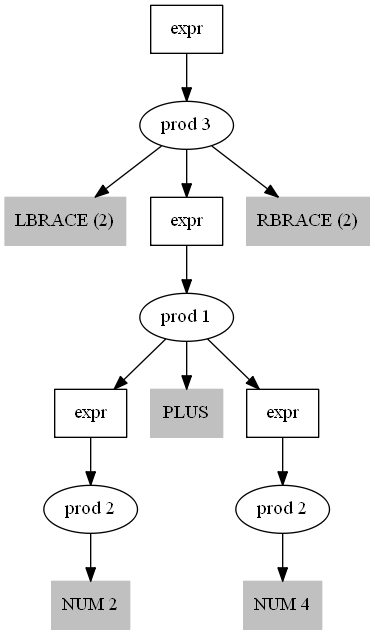
\includegraphics[height=100mm]{Pictures/Dynamic_StaticRes2.png}
    \end{subfigure}
    \caption{Результат алгоритма для статической подсветки.}
    \label{staticRes}
\end{figure}

Предположим, что каретка курсора находится непосредственно перед токеном LBRACE (1). Тогда в зависимости от пути во входном графе парными этому токену будут являться RBRACE (1) или RBRACE(2). Поэтому нужно вернуть два дерева разбора. Одно должно содержать токены LBRACE(1) и RBRACE(1), а другое ~-- токены LBRACE(1) и RBRACE(2) (см. рис. ~\ref{dynamicRes}). Заметим при этом, что наличие других токенов (например, LBRACE 2) нас особо не интересует. Лишь бы получилось корректное синтаксическое дерево, соответствующее некоторому пути во входном графе.

\begin{figure}[h]
    \centering
    \begin{subfigure}[h]{0.25\textwidth}
        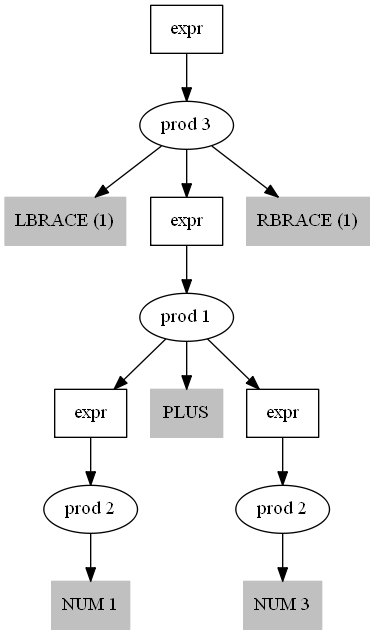
\includegraphics[height=100mm]{Pictures/Dynamic_DynamicRes1.png}
    \end{subfigure}
    \qquad \qquad
    \begin{subfigure}[h]{0.25\textwidth}
        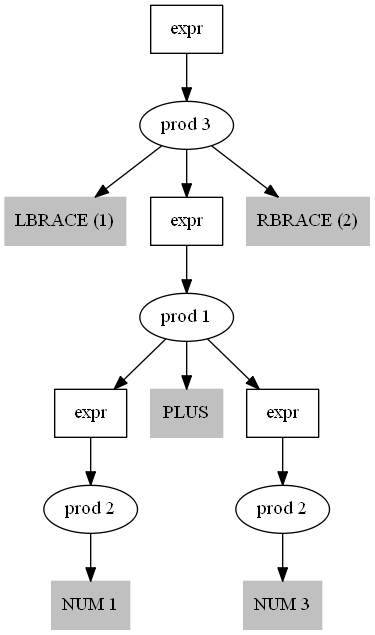
\includegraphics[height=100mm]{Pictures/Dynamic_DynamicRes2.png}
    \end{subfigure}
    \caption{Результат алгоритма для динамической подсветки.}
    \label{dynamicRes}
\end{figure}

Таким образом, если курсор стоит перед парным токеном, то нам нужно вернуть ровно n деревьев, где n ~-- количество пар данного токена. 

Поскольку алгоритмы во многом пересекаются, решено было модифицировать алгоритм для статической подсветки следующим образом. 

В качестве входа алгоритм принимает два параметра:
\begin{itemize}
\item root ~-- корень графа разбора;
\item токен t, пары которому нужно найти.
\end{itemize}

В ходе своей работы алгоритм сохраняет полученные деревья в множестве trees. Как и в предыдущем алгоритме, все вершины окрашены в белый цвет.

Алгоритм возвращает GetAllTreesWithToken (root, token).

GetAllTreesWithToken (root, token):
\begin{enumerate}
\item trees = $\emptyset$
\item newTree = Handle (root, token, trees)
\item пока newTree $\notin$ trees:
\item \qquad trees = trees $\cup$ \{newTree\}
\item \qquad newTree = Handle (root, token, trees)
\item вернуть trees
\end{enumerate}		
		
Handle (v, token, trees):
\begin{enumerate}
\item Если вершина v - вершина-символ, то 
    \begin{itemize}
        \item если OutEdges (v) == 1, то Handle (Succ (v), token, trees).
        \item если OutEdges (v) > 1, то если среди u $\in$ Succ(v) $\exists$ s такой, что token $\in$~Tokens (s), то Handle (s, token, trees). 
        \item Иначе идти по такому r $\in$ Succ(v), который содержит наибольшее количество новых токенов (на фоне множества trees). 
	\end{itemize}
	Перейти к шагу 3.
\item Если текущая вершина - вершина-продукция, то для каждой вершины u из Succ(v) сделать следующее:  Handle (u, token, trees). Перейти к шагу 3.
\item Покрасить v в чёрный цвет. Если v == root, то перейти к шагу 4.
\item Алгоритм завершает работу. Вернуть дерево, состоящее из “чёрных” вершин. 
\end{enumerate}

Иллюстрация работы алгоритма продемонстрирован на рисунке ~\ref{ex}.

\begin{figure}[h]
    \centering
    % \begin{subfigure}[h]{0.25\textwidth}
    %     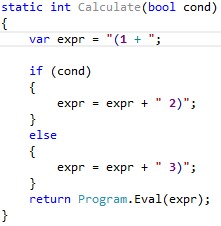
\includegraphics{Pictures/BracketExampleWithoutCaret.PNG}
    %     \caption*{Без курсора.}
    % \end{subfigure}
    % \\
    \begin{subfigure}{0.25\textwidth}
        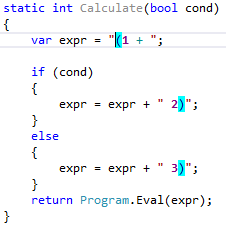
\includegraphics{Pictures/BracketExample.png}
        \caption*{Курсор перед открывающей скобкой.}
    \end{subfigure}
    \qquad \qquad \qquad
    \begin{subfigure}{0.25\textwidth}
        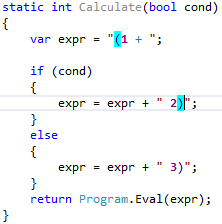
\includegraphics{Pictures/BracketExampleWithRight.png}
        \caption*{Курсор после закрывающей скобки.}
    \end{subfigure}
    \caption{Иллюстрация работы алгоритма с подсветкой скобок.}
    \label{ex}
\end{figure}